\section{Instance Layout}

\begin{figure}
    \begin{minipage}{.35\textwidth}
        \centering
        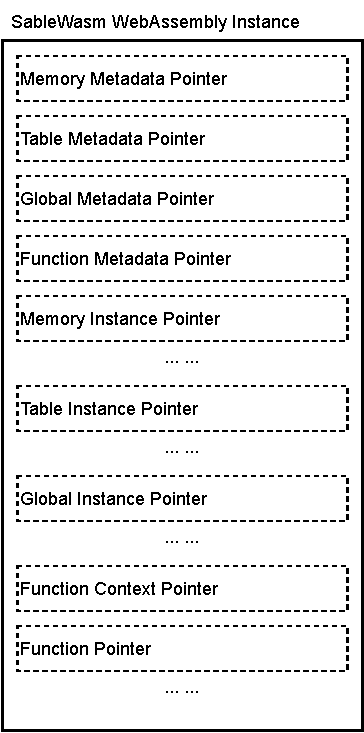
\includegraphics[
            width=\textwidth
        ]{Images/5.Backend and Runtime/instance}
    \end{minipage}\hfill
    \begin{minipage}{.6\textwidth}
        \begin{lstlisting}[
            language=C, 
            basicstyle=\linespread{1}\ttfamily\footnotesize]
struct instance {
    memory_metadata_t   *memory_metadata;
    table_metadata_t    *table_metadata;
    global_metadata_t   *global_metadata;
    function_metadata_t *function_metadata;
    memory_t            *memories[NUM_MEMORY];
    table_t             *tables[NUM_TABLE];
    global_t            *globals[NUM_GLOBAL];
    struct {
        struct instance *context;
        function_t      *function_ptr;
    } *functions[NUM_FUNCTIONS];
};        
    \end{lstlisting}
    \end{minipage}
    \caption{SableWasm WebAssembly instance}
    \label{fig:backend-instance}
\end{figure}

This section discusses the WebAssembly instance implementation in SableWasm.
A WebAssembly instance hosts all the runtime structures that the generated
shared libraries require, such as linear memories and indirect tables.
Figure~\ref{fig:backend-instance} illustrates the design of the WebAssembly
instance. SableWasm's WebAssembly instance object consists of two parts,
metadata entries and entity pointers. One may also notice that the instance
object's size may vary from one module to another depending on how many entities
are declared. This behaviour is intentional by design. The SableWasm runtime
system needs to compute the address of the pointers based on the metadata
information on the fly. By packing all pointers in a consecutive memory region,
we reduce one layer of indirection for the runtime system, and in theory, may
improve runtime performance. On the other hand, the generated shared library
has all the entities address inlined as the backend can compute them during code
generation, which does not incur any performance loss. For most of the entities,
they are pretty straightforward, and we will skip the discussion here. In the
rest of the section, we focus on three aspects: the metadata entries,
the function entity representations, and the instance initialization protocol
in SableWasm.

\paragraph{Metadata}
One could think of the metadata as the signatures for entities, and indeed, the
SableWasm runtime system prepares the instance object based on the metadata.
Further, shared libraries generated by SableWasm only publicly expose the
metadata and initialization function to conceal module details. Metadata encodes
the type for the entity. For linear memories and indirect tables, this is
relatively trivial as their types only consist of an integer pair. In the case
of global variables, things are a little bit complicated. A quick reminder,
WebAssembly global variable types keep track of their value type and mutability.
The first problem here is how to encode WebAssembly value types. One solution is
to use WebAssembly value type binary format. However, this encoding strategy is
hard to maintain as a human cannot directly read them. Here we use the JVM
approach for value type encoding
\footnote{\url{https://docs.oracle.com/javase/7/docs/technotes/
        guides/jni/spec/types.html}}. In short, in SableWasm, we encode
32-bit integers as `I', 64-bit integers as 'J', single-precision floating-point
numbers as 'F', double-precision floating-point numbers as 'D', and finally,
128-bit vectors as 'V'. The second problem is how to encode mutability. In
SableWasm, we use capital letters for constant global variable types and lower
letters for mutable ones. Finally, for function types, we follow a similar
design as we used for global variables. SableWasm encodes a function type into a
null-terminated string. Let's take \texttt{[i32, f32] -> [v128]} as an example.
SableWasm encodes the type into `\texttt{IF:V}'. The colon acts as a separator
between parameter types and result types. Note that `\texttt{:}' itself is also
a valid SableWasm function signature string, and represents \texttt{[] -> []},
a void function with no arguments. Finally, metadata also encodes module names
and entity names for import entities and names for export entities, which play
a critical role later in the module initialization phase.

\paragraph{Function entity representation}
The WebAssembly specification classifies the functions into two groups,
WebAssembly functions and host functions. WebAssembly functions are any
functions defined within a WebAssembly module. On the other hand, host
functions are directly provided by the host system, and from the WebAssembly
module's perspective, the host functions are black boxes without any knowledge
of their internals. Making things more complex, in MVP WebAssembly, there are no
explicit requirements on how the WebAssembly functions should behave if they
are invoked from other modules. Here we use a similar generalization like the
one adopted by Javascript \footnote{WebAssembly Javascript Interface:
    \url{https://www.w3.org/TR/wasm-js-api-1/}}. In short, in SableWasm, if a
module exports a function, it exports the function in a closure that captures
its enclosing instance. Suppose a second module invokes the exported closure
as an import function. In this case, the function still only has access to its
original module's entities and only communicates to the second module via
return values. Hence, in SableWasm, we implement our function as a pair of
pointers. The first one refers to its enclosing instance, and the second one
relates to the generated function code. In this chapter's introduction, we
mentioned that we pass the instance object as the first argument to the
generated functions upon function calls. But, what should we give to the host
function invocations? SableWasm defines that for all the host functions, the
instance object pointer will always point to the caller's enclosing instance
so that the host functions can access the internals of the caller's module.

\paragraph{Initialization protocol}
In the last part of the section, we will cover the initialization protocol we
used in SableWasm. The initialization protocol consists of three basic steps:
validation, instance preparation, and initialization.
In the validation phase, we load the shared library with the operating system's
help, such as \texttt{dlopen} on Linux, and check if it contains all the
required symbols. Currently, a SableWasm shared library needs to export five
symbols in total. Table~\ref{tbl:sablewasm-runtime-export-syms} illustrates the
symbols expected from the generated shared libraries. The instance initializer
function takes a \emph{prepared} instance object as the argument. The next step
in SableWasm is to construct this \emph{prepared} instance object. The idea of
a \emph{prepared} instance object is that we want to separate the memory
allocation from the value initialization. In SableWasm, the runtime system
handles the memory allocation, while on the other hand, the initializer function
takes care of the value initialization. In the second phase, the SableWasm
runtime allocates all the entities and attaches them to the module instance.
Note that SableWasm also resolves all the import names at this stage, and it
will only proceed to the next step if all the expecting import entities are set.
The import name binding utilizes the module names and entity names provided by
the metadata. Finally, the last step is the initialization. SableWasm will
invoke the initializer function supplied by the shared library. The initializer
function takes care of all kinds of value initialization, such as setting values
for global variables and copying data segments into linear memories. If the
runtime system adequately prepares the instance context, the initializer
function should never fail.

\begin{table}[h]
    \centering
    \begin{tabular}{|l|l|}
        \hline
        \textbf{Symbol Name}          & \textbf{Description}          \\ \hline
        \_\_sable\_global\_metadata   & Metadata for global values    \\ \hline
        \_\_sable\_memory\_metadata   & Metadata for linear memories  \\ \hline
        \_\_sable\_table\_metadata    & Metadata for indirect tables  \\ \hline
        \_\_sable\_function\_metadata & Metadata for functions        \\ \hline
        \_\_sable\_initialize         & Instance initializer function \\ \hline
    \end{tabular}
    \caption{SableWasm shared libraries exported symbols}
    \label{tbl:sablewasm-runtime-export-syms}
\end{table}